\documentclass[12pt,a4paper]{article}

\usepackage[T2A]{fontenc}
\usepackage[utf8]{inputenc}
\usepackage[english,russian]{babel}

\usepackage{amsmath}

\usepackage{geometry}
\usepackage{graphicx}
\usepackage{float}
\usepackage{caption}

\captionsetup[figure]{
    name=Рисунок,
    labelsep=period
}

\geometry{
    left=20mm,
    right=20mm,
    top=20mm,
    bottom=20mm
}

\usepackage{xurl}
\usepackage[
    colorlinks=true,
    linkcolor=black,
    urlcolor=blue,
    citecolor=black
]{hyperref}

\urlstyle{same}
\usepackage{enumitem}

\begin{document}

\noindent УДК 004.514

\vspace{0.5cm}

Журавлев Д.С.

МИРЭА -- Российский технологический университет, Москва, Россия

Научный руководитель: Андрианова Е.Г.

\vspace{0.5cm}

\begin{center}
\textbf{
РЕКОМЕНДАТЕЛЬНЫЙ ПОДХОД К МОДИФИКАЦИИ
ПОЛЬЗОВАТЕЛЬСКОГО ИНТЕРФЕЙСА НА ОСНОВЕ
АНАЛИЗА ТРЕКИНГА ВЗГЛЯДА И АНАЛИТИЧЕСКИХ МЕТРИК
}
\end{center}

\vspace{0.3cm}

\noindent
\textbf{Аннотация.}
Статья посвящена рассмотрению рекомендательного подхода к модификации
пользовательского интерфейса на основе анализа направления взгляда пользователя.
Предлагаемый метод основан на использовании нейросетевой модели предсказания
координат взгляда по данным видеопотока с веб-камеры, построении тепловых карт
внимания и применении аналитических метрик для количественной оценки визуального
поведения. В работе используются коэффициент корреляции тепловых карт, матрицы
несоответствия и визуальные показатели траекторий и фиксаций взгляда для сравнения
сценариев взаимодействия с интерфейсом до и после его изменения. Экспериментальная
апробация демонстрирует возможность объективной оценки удобства интерфейса и
формирования обоснованных рекомендаций по его модификации.

\vspace{0.3cm}

\noindent
\textbf{Ключевые слова:}
пользовательский интерфейс, трекинг взгляда, нейросеть,
анализ поведения пользователя.

\vspace{0.8cm}

\noindent
Zhuravlev D.S.

\vspace{0.3cm}

\begin{center}
\textbf{
A RECOMMENDATION APPROACH TO USER INTERFACE MODIFICATION
BASED ON EYE-TRACKING ANALYSIS AND ANALYTICAL METRICS
}
\end{center}

\vspace{0.3cm}

\noindent
\textbf{Abstract.}
This article examines a recommendation approach for user interface modification
based on user gaze analysis. The proposed method relies on a neural network model
for predicting gaze coordinates based on webcam video stream data, constructing
attention heatmaps, and applying analytical metrics to quantify visual behavior.
The study utilizes heatmap correlation coefficients, disparity matrices, and visual
indicators of gaze trajectories and fixations to compare interaction scenarios with
the interface before and after its modification. Experimental testing demonstrates
the feasibility of objectively assessing interface usability and generating informed
recommendations for its modification.

\vspace{0.3cm}

\noindent
\textbf{Key words:}
user interface, eye tracking, neural network, user behavior analysis.

\vspace{0.8cm}

В условиях активного развития информационных систем и усложнения
программных продуктов особую актуальность приобретает задача оценки
удобства пользовательских интерфейсов. От того, насколько интуитивно
понятен интерфейс, зависит скорость освоения системы, количество
совершаемых пользователем ошибок и общая эффективность работы с
программным продуктом. Традиционно оценка удобства интерфейса
основывается на анализе времени выполнения действий, количестве кликов,
а также на результатах опросов и анкетирования пользователей. Однако
подобные методы позволяют судить лишь о конечном результате
взаимодействия, не раскрывая особенностей восприятия интерфейса
в процессе работы.

Пользовательский интерфейс воспринимается человеком прежде всего
визуально, и именно распределение внимания по элементам экрана
определяет характер взаимодействия с системой. Взгляд пользователя
отражает его когнитивные процессы, указывает на зоны повышенного
интереса, затруднений или неопределённости~[1]. Анализ визуального
поведения позволяет получить более глубокое понимание того, как
пользователь ориентируется в интерфейсе, какие элементы привлекают
внимание в первую очередь, а какие остаются незамеченными.

Использование данных о направлении взгляда открывает возможность
перехода от субъективной оценки удобства интерфейса к количественно
обоснованному анализу. Трекинг взгляда позволяет фиксировать не только
факт выполнения действия, но и путь, которым пользователь приходит
к этому действию, что особенно важно при исследовании сложных
сценариев взаимодействия~[2]. Таким образом, возникает необходимость
разработки методов, позволяющих использовать информацию о визуальном
поведении пользователя для последующей оценки и модификации интерфейса.

Проблема заключается в том, что сами по себе данные трекинга взгляда
являются лишь набором координат, требующим последующей интерпретации
и аналитической обработки. Для практического применения необходимо
сформировать подход, который позволил бы на основе этих данных делать
выводы о степени удобства интерфейса и формировать рекомендации
по его изменению. Именно решение данной задачи и определяет направление
рассматриваемого исследования.

Переход к анализу направления взгляда как инструменту оценки интерфейса
обусловлен тем, что визуальное восприятие является первичным этапом
взаимодействия пользователя с системой. Прежде чем выполнить какое-либо
действие, пользователь сканирует экран, выделяет значимые элементы,
соотносит их с поставленной задачей и только после этого принимает решение
о дальнейших действиях. Этот процесс происходит естественно и зачастую
неосознанно, однако именно он отражает реальную сложность или,
напротив, интуитивность интерфейса.

В отличие от анализа кликов и времени выполнения операций, данные
о взгляде позволяют наблюдать не только итоговое действие, но и путь,
которым пользователь к нему приходит. Траектория движения взгляда,
длительность фиксаций на отдельных элементах и последовательность
их просмотра формируют уникальный паттерн визуального поведения,
который может быть использован для оценки того, насколько предсказуемо
и логично организован интерфейс. Если пользователь тратит значительное
время на поиск нужного элемента или неоднократно возвращается к одним
и тем же зонам экрана, это может свидетельствовать о перегруженности
интерфейса или недостаточной наглядности расположения элементов.

Таким образом, анализ направления взгляда предоставляет качественно
новый уровень информации о взаимодействии пользователя с интерфейсом.
Он позволяет выявить скрытые проблемы навигации, определить зоны
повышенной когнитивной нагрузки и получить объективные данные
о распределении внимания. Это делает трекинг взгляда перспективным
инструментом для формирования рекомендаций по модификации интерфейса
и повышения его удобства.

Определение направления взгляда пользователя основывается на анализе
изображения его лица, получаемого с помощью стандартной веб-камеры.
В каждый момент времени видеопоток содержит информацию о положении глаз
и ориентации головы, которые в совокупности позволяют оценить, в какую
часть экрана направлено внимание пользователя. Такой подход не требует
специализированного оборудования и может быть реализован с использованием
методов компьютерного зрения и математической обработки изображений.
Пример базовой работы программы с пользователем представлен
на рисунке~\ref{fig:program}, а процесс сбора данных ---
на рисунке~\ref{fig:coordinates}.

\begin{figure}[H]
    \centering
    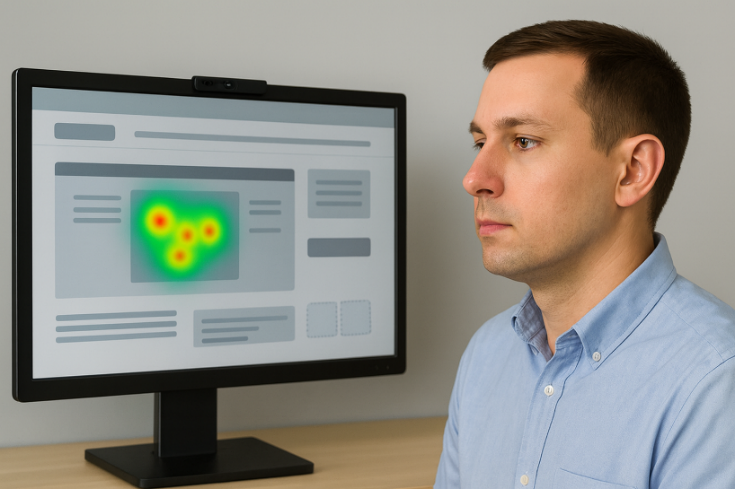
\includegraphics[width=0.8\textwidth]{figures/figure1.png}
    \caption{Базовая работа программы и пользователя через камеру}
    \label{fig:program}
\end{figure}

\begin{figure}[H]
    \centering
    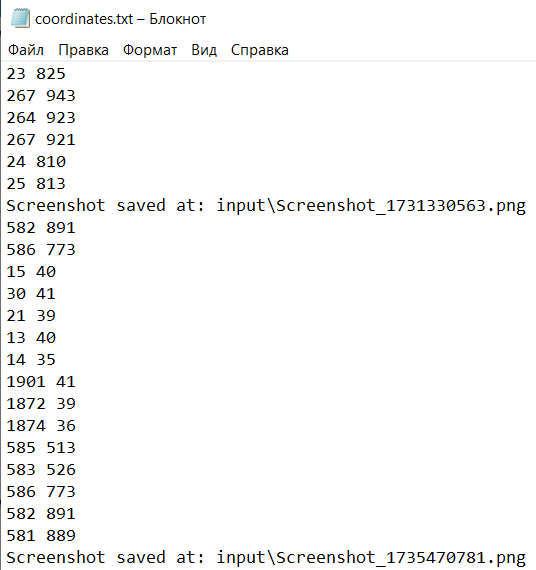
\includegraphics[width=0.7\textwidth]{figures/figure2.png}
    \caption{Сбор данных координат взгляда пользователя в единый датасет}
    \label{fig:coordinates}
\end{figure}

На первом этапе из видеопотока выделяются ключевые ориентиры лица,
позволяющие определить положение глаз, границы глазных щелей и
относительное положение зрачков. Дополнительно учитываются параметры
ориентации головы, отражающие её поворот и наклон относительно камеры.
Эти данные формируют набор числовых признаков, описывающих текущее
состояние глаз пользователя и положение его головы.

Полученные признаки подаются на вход обучаемой модели, предназначенной
для предсказания координат точки взгляда на экране. Модель устанавливает
зависимость между положением глаз и головы и соответствующей точкой
на экране, на которую смотрит пользователь. Для повышения точности
используется предварительный этап калибровки, в ходе которого пользователь
последовательно фиксирует взгляд на контрольных точках, что позволяет
сформировать индивидуальный набор данных для обучения модели~[3].

Таким образом, направление взгляда определяется не напрямую по изображению
экрана, а косвенно --- через анализ положения глаз и ориентации головы.
Это позволяет получать устойчивые предсказания координат взгляда
в реальном времени и использовать их в дальнейшем для анализа визуального
поведения пользователя при работе с интерфейсом.

Последовательность предсказанных координат взгляда во времени образует
непрерывный поток данных, который может быть преобразован в более
наглядные и информативные представления визуального поведения пользователя.
Одним из таких представлений являются тепловые карты внимания, формируемые
на основе частоты попадания взгляда в различные области экрана. Каждая
точка взгляда увеличивает «интенсивность» соответствующей области, что
позволяет визуально выделить зоны, на которые пользователь обращает
наибольшее внимание в процессе работы с интерфейсом.

Тепловые карты дают обобщённое представление о распределении внимания
и позволяют определить наиболее просматриваемые элементы, а также области,
которые остаются практически незамеченными. Это особенно важно при анализе
сложных интерфейсов, где расположение элементов может не соответствовать
ожиданиям пользователя. Наглядность тепловых карт делает их удобным
инструментом для первичного анализа и сравнения различных вариантов
интерфейса.

Помимо обобщённого распределения внимания важную роль играет анализ
фиксаций взгляда. Фиксацией считается устойчивое удержание взгляда
в пределах небольшой области экрана в течение определённого промежутка
времени. Количество и продолжительность фиксаций на конкретных элементах
интерфейса позволяют судить о степени их значимости для пользователя,
а также о возможных затруднениях при восприятии информации.

Дополнительную информацию предоставляет анализ траекторий взгляда,
представляющих собой последовательность перемещений между точками фиксации.
Траектория отражает логику навигации пользователя по интерфейсу:
последовательность просмотра элементов, возвраты к уже просмотренным
областям и общий путь, который проходит взгляд до выполнения целевого действия~[4].
Сравнение траекторий в различных условиях позволяет выявлять
различия в стратегии взаимодействия и оценивать влияние изменений
интерфейса на поведение пользователя.

Пример тепловой карты с отображением фиксаций и траектории движения взгляда
пользователя представлен на рисунке~\ref{fig:heatmap}.

\begin{figure}[H]
    \centering
    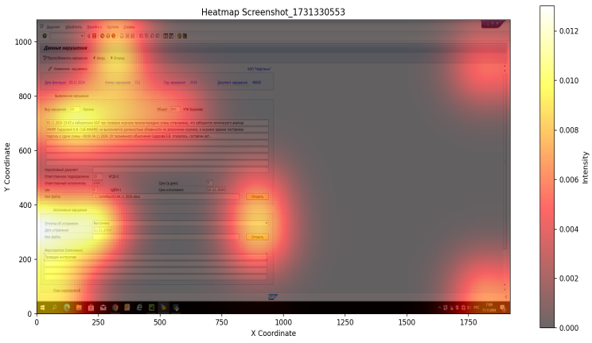
\includegraphics[width=0.8\textwidth]{figures/figure3.png}
    \caption{Пример тепловой карты распределения внимания пользователя на интерфейсе}
    \label{fig:heatmap}
\end{figure}

Для перехода от наглядных визуальных представлений к количественной
оценке удобства интерфейса используются аналитические метрики,
позволяющие сравнивать визуальное поведение пользователей в различных
условиях. В качестве таких метрик применяются коэффициент корреляции
тепловых карт и матрицы несоответствия, отражающие корректность
распознавания пользовательских сценариев по паттернам взгляда.

Коэффициент корреляции используется для сравнения тепловых карт,
полученных в разных группах пользователей или при различных вариантах
интерфейса. Каждая тепловая карта может быть представлена в виде набора
числовых значений, соответствующих интенсивности внимания в отдельных
областях экрана. Сравнение этих значений позволяет оценить степень
сходства распределения внимания. Высокое значение корреляции
свидетельствует о том, что пользователи воспринимают интерфейс схожим
образом, а низкое --- указывает на различия в навигации и распределении
внимания. Данная метрика позволяет объективно оценивать изменения
интерфейса и их влияние на визуальное поведение.

Дополнительно для оценки используется построение матриц несоответствия.
Каждый запуск пользовательского сценария рассматривается как отдельное
наблюдение, для которого определяется, насколько визуальное поведение
соответствует ожидаемому паттерну. В качестве критерия используется
пороговое значение корреляции с эталонной тепловой картой. Если значение
превышает заданный порог, сценарий считается корректно распознанным,
в противном случае --- некорректным. На основе сравнения фактических
и ожидаемых результатов формируются значения истинно положительных,
ложноположительных, ложноотрицательных и истинно отрицательных случаев.

Использование данных метрик позволяет перейти от субъективной
интерпретации тепловых карт к строгой количественной оценке удобства
интерфейса. Корреляция отражает степень предсказуемости визуального
восприятия, а матрицы несоответствия --- способность системы распознавать
корректность выполнения сценариев по поведению пользователя.
Совместное применение этих показателей создаёт основу для обоснованных
выводов о необходимости модификации интерфейса.

Практическое применение описанного подхода реализуется в форме серии
экспериментов, в которых пользователи выполняют заранее определённые
сценарии взаимодействия с интерфейсом. Каждый сценарий предполагает
последовательность действий, направленных на достижение конкретной цели,
что позволяет наблюдать устойчивые паттерны визуального поведения.
В ходе выполнения сценариев фиксируются координаты взгляда, на основе
которых формируются тепловые карты, траектории и данные о фиксациях.

Экспериментальная схема предполагает сравнение двух состояний интерфейса:
исходного варианта и варианта после внесения изменений. Пользователи
выполняют одни и те же сценарии в обоих случаях, что обеспечивает
сопоставимость полученных данных. Для повышения достоверности результатов
каждый сценарий выполняется многократно различными пользователями
с разным уровнем опыта работы с системой.

Полученные данные подвергаются аналитической обработке. Для каждого
запуска строится тепловая карта и рассчитывается её корреляция
с эталонным распределением внимания. На основании этого принимается
решение о корректности распознавания сценария, после чего формируются
матрицы несоответствия. Дополнительно анализируются время поиска целевых
элементов, количество фиксаций и особенности траектории взгляда.

Сравнение результатов до и после модификации интерфейса позволяет
количественно оценить влияние внесённых изменений на визуальное
поведение пользователей. Такая экспериментальная схема обеспечивает
объективность выводов и демонстрирует практическую применимость
предложенного подхода при анализе и улучшении пользовательских
интерфейсов.

Завершающим этапом применения предложенного подхода является формирование
рекомендаций по модификации пользовательского интерфейса на основе
полученных аналитических данных. В отличие от субъективных оценок,
основанных на мнении пользователей или разработчиков, рекомендации
в данном случае опираются на объективные показатели визуального
поведения и количественные метрики.

Анализ тепловых карт позволяет выявить области интерфейса, которые
привлекают избыточное внимание или, напротив, остаются незамеченными.
Если пользователи длительное время фиксируют взгляд в определённых
зонах без выполнения целевого действия, это может свидетельствовать
о перегруженности интерфейса или недостаточной наглядности расположения
элементов. Аналогично, зоны, на которые практически не направляется
взгляд, могут указывать на неэффективное размещение важной информации.

Корреляционный анализ и матрицы несоответствия дополняют визуальную
оценку, позволяя количественно подтвердить наличие проблемных участков
интерфейса. Снижение корреляции и увеличение количества ложных
распознаваний сценариев указывают на необходимость изменения структуры
или расположения элементов. В свою очередь, улучшение данных показателей
после внесения изменений подтверждает правильность выбранного направления
модификации.

Таким образом, результаты анализа визуального поведения трансформируются
в конкретные рекомендации: упрощение перегруженных областей,
перераспределение ключевых элементов, оптимизация навигационных переходов
и повышение наглядности интерфейса. Предложенный подход позволяет
не только выявлять существующие проблемы, но и обосновывать необходимость
изменений на основе количественных данных, что делает процесс модификации
интерфейса более целенаправленным и обоснованным.

////Чисто для математической формулы в статье, вставляю от себя данный фрагмент 
(и еще немного текста):

\begin{equation}
P_n(x) =
\sum_{i=0}^{n}
y_i
\prod_{\substack{j=0 \\ j \neq i}}^{n}
\frac{x - x_j}{x_i - x_j},
\label{eq:lagrange}
\end{equation}

где $x_i$ --- узлы интерполяции, $y_i$ --- соответствующие значения
функции, а $P_n(x)$ --- интерполяционный полином степени не выше $n$.

////Конец вставки моей формулы и текста 

\bigskip
\noindent\textbf{Список литературы}

{\sloppy
\begin{enumerate}[label=\arabic*), leftmargin=1.8em, itemsep=0.4em]

    \item Eye-tracking as a tool for researching user behavior (2025).
    URL: \url{https://www.researchgate.net/publication/381633551_Eyetracking_as_a_tool_for_researching_user_behavior}
    (Дата обращения 10.02.2026)

    \item Eye-tracking исследования (айтрекинг) --- обзор современного метода
    UX-анализа (UsabilityLab, 2025).
    URL: \url{https://usabilitylab.ru/uxmethods/testingmethods/eye-tracking-issledovaniya/}
    (Дата обращения 08.02.2026)

    \item Расширение метода окулографического пространственного мониторинга
    с использованием мультимодальной CNN с геометрическими признаками (2025).
    URL: \url{http://injoit.org/index.php/j1/article/download/2358/2019}
    (Дата обращения 09.02.2026)

    \item Онлайн статья «20 эффективных методов UX/UI-исследований»
    (FOQUZ, 2025).
    URL: \url{https://foquz.online/blog/top-20-ux-ui-research-methods}
    (Дата обращения 10.02.2026)

\end{enumerate}
}

\end{document}